\section{Result and Discussion}

\subsection{Final Results}
This section presents the results of comparing four optimization strategies on the ARES Experimental Area beam 
tuning problem including Nelder-Mead, standard BO, BO\_prior (mismatched), and BO\_prior (matched\_prior\_newtask).  All experiments were run for 100 iterations over 10 independent trials. \

\begin{figure}[ht]
    \centering
    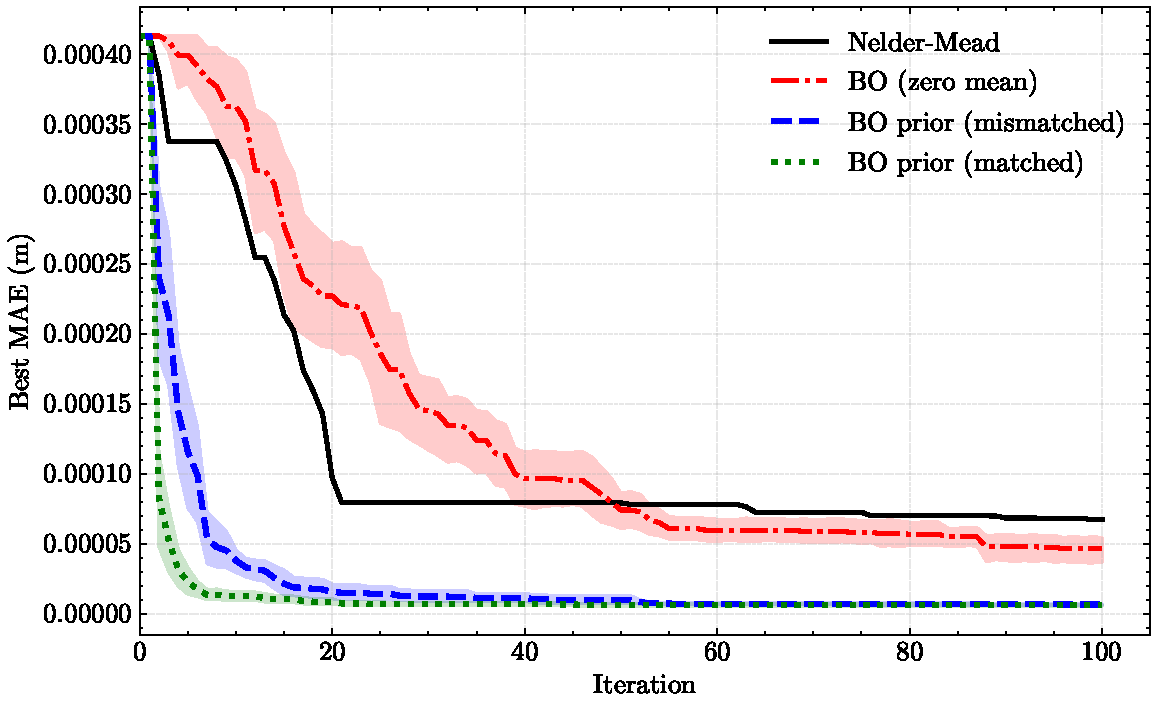
\includegraphics[width=0.8\textwidth]{figures/convergence_curves.pdf}
    \caption{Convergence curve showing the cumulative minimum MAE over iterations for each optimization strategy.}
    \label{fig:convergence_curve}
    
\end{figure}

The plot’s most interesting insight is how fast the are the two physics informed variants of BO from the other optimizers. 
The matched prior (green dotted line) drops sharply within the first five iterations, and flattens out by iteration 10 already. 
The mismatched prior (blue dashed line) is only slightly behind the matched case which makes sense because the GP needs some observations 
before the optimizer can start correcting the misalignment parameters, thus this case takes roughly 15 iterations to reach a comparable 
level to the matched case. The trajectory of standard BO with zero mean (red dashed-dot line) is somewhat more gradual. It does improve 
steadily, but even by iteration 60 , it is still clearly above the physics informed methods. Additionally, the broad shaded region of 
uncertainty band also indicates that different trials converge at quite different rates reflecting the fact that without any guidance from prior, 
the initial random exploration phase can either go well or poorly, depending nowhere those few points happen to land. Nelder-Mead (solid black line) 
displays an interesting pattern. In the early phase (around iterations 10-20), it actually decreases more quickly than normal BO, which is the 
characteristics of the simplex method to make large directed steps once it finds a downhill direction. However, it plateaus around  80 $\mu$m and then never 
goes lower than that. This shows that in a five dimensional space with a complex landscape, the simplex might get stuck in local minima or lose its shape and 
thus, without a probabilistic model to guide exploration, it has no mechanism to escape.


%\section{Summary Performance Metrics}
%\label{sec:metrics}

%Table~\ref{tab:results_main} collects the key performance metrics across all four methods. These numbers correspond to the evaluation protocol described in Section~3.5 and are directly comparable to the results reported in~\cite{kaiser2024rl}.

\begin{landscape}
\centering
\vspace*{\fill}
\begin{table}[H]
\centering
\caption{Performance of optimisation algorithms on ARES beam tuning in simulation (100 iterations, 10 trials). The target threshold for steps to target and success rate is \SI{40}{\micro\metre}.}
\label{tab:results_main}
\small
\renewcommand{\arraystretch}{1.3}
\begin{tabular}{l cc cc cc cc c}
\toprule
 & \multicolumn{2}{c}{\textbf{Final error} ($\boldsymbol{\mu}$\textbf{m})} & \multicolumn{2}{c}{\textbf{RMSE} ($\boldsymbol{\mu}$\textbf{m})} & \multicolumn{2}{c}{\textbf{Improvement} (\%)} & \multicolumn{2}{c}{\textbf{Steps to target}} & \\
\cmidrule(lr){2-3} \cmidrule(lr){4-5} \cmidrule(lr){6-7} \cmidrule(lr){8-9}
\textbf{Optimiser} & Median & Mean & Median & Mean & Median & Mean & Median & Mean & \textbf{Success rate} \\
\midrule
Nelder-Mead           & 67  & $67 \pm 0$     & 149 & $149 \pm 0$    & 84  & $84 \pm 0$   & ---  & ---            & 0\%   \\
BO (zero mean)        & 46  & $46 \pm 15$    & 179 & $181 \pm 18$   & 89  & $89 \pm 4$   & 82   & $82 \pm 6$     & 20\%  \\
BO + prior (mismatch) & 6   & $7 \pm 2$      & 71  & $73 \pm 8$     & 98  & $98 \pm 0$   & 14   & $13 \pm 5$     & 100\% \\
BO + prior (matched)  & 6   & $6 \pm 1$      & 60  & $60 \pm 1$     & 99  & $99 \pm 0$   & 4    & $4 \pm 1$      & 100\% \\
\bottomrule
\end{tabular}
\end{table}
\vspace*{\fill}
\end{landscape}

As we can see from the final computed table, the final error (mae) for both physics informed BO variants achieve a median of 6$\mu$m, 
which is better than Nelder-Mead(67$\mu$m) and standard BO(46$\mu$m). In practical terms, 6$\mu$m is well below the 20$\mu$m effective 
resolution of ARES diagnostic screen, so the optimizer has effectively pushed the beam to the best state that could be measured by an 
actual machine. Similarly, for the Improvement percentage,  strating from the same MAE of roughly 413$\mu$m, the physics based approaches 
minimize the error by over 98\%, whereas standard BO manages about 89\% and Nelder-Mead about 84\%. 
Even the standard deviations also shows worth noticing results, the physics informed results are remarkably consistent across trials, 
whereas standard BO has a spread of $\pm$4, which confirms that the visual impression from the convergence curves plot that it is more 
sensitive to initial exploration phase. The success rate and steps to target columns shows quite impressive results as well. 
Setting the target of 40$\mu$m (which is a reasonable threshold set for a good enough beam quality), both physics informed BO variants 
reach it in every single trials making it a success rate of 100\%, where the matched prior scenario gets there in just 4 steps and mismatched 
prior scenario gets there in 14 steps. The standard BO only succeeds in 2 out of 10 trials making a success rate of 20\% and when it works, 
it requires a median of 82 steps. Nelder-Mead never reaches the target within the 100 steps budget. \

Methods that spend a lot of iterations at high MAE values before converging are penalized by the RMSE metric. The RMSE metric also shows 
how both variants of  physics informed BO are better than the baseline methods. The matched prior BO has the lowest RMSE (60$\mu$m), 
reflecting the fact that it starts producing good predictions from the very first steps. The mismatched prior BO is slightly higher 
(71$\mu$m), since it spends a few early iterations adjusting its internal model. Nelder-Mead and standard BO both have RMSE values 
exceeding 140 $\mu$m due to their long initial phase where they are still exploring. 

\begin{figure}[ht]
    \centering
    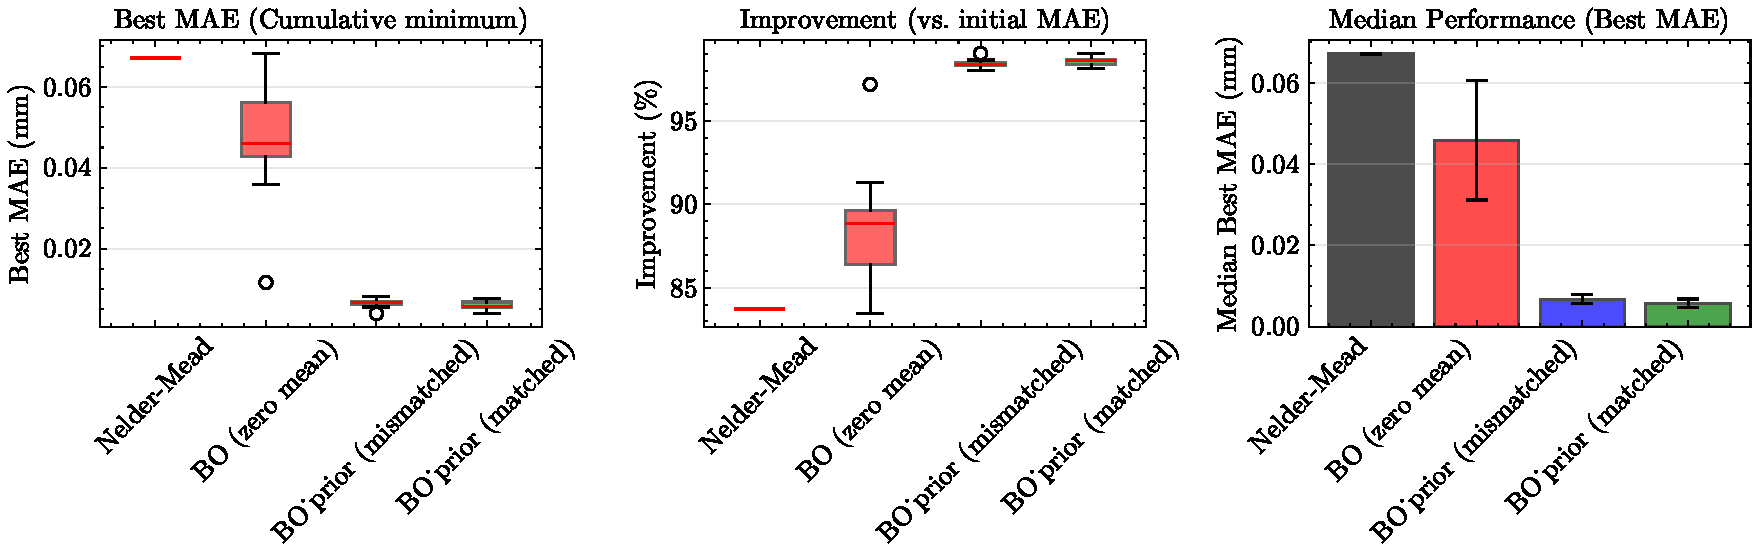
\includegraphics[width=0.8\textwidth]{figures/boxplot_comparison.pdf}
    \caption{Box plot comparison across 10 trials. Left: final MAE (best achieved) for each
method. Centre: percentage improvement from the initial beam state. Right: median
final MAE with standard deviation error bars.}
    \label{fig:boxplot_comparison}
    
\end{figure}

Figure4.2 breaks down how each method performed on a per trial basis. In the left panel, 
Nelder-Mead collapses to a single line at 67$\mu$m, indicating that it is getting stuck to 
the same local minima every time. Standard BO shows a wide box ranging from 25$\mu$m to 60 $\mu$m with 
one lucky outlier near 10 $\mu$m, whereas both the physics informed BO variants sit tightly around 
6 $\mu$m. The central panel confirms that teh prior based BO methods cluster above 98\% improvements,
 BO scatters between 84\% and 97\% whereas Nelder-Mead stays below 84\%. And finally the right panel’s median 
 bars make the order of magnitude gap clearly visible. Figure 4.3 provides another perspective by plotting each 
 trials’s final MAE against how many steps it took to converge. 

 
\begin{figure}[ht]
    \centering
    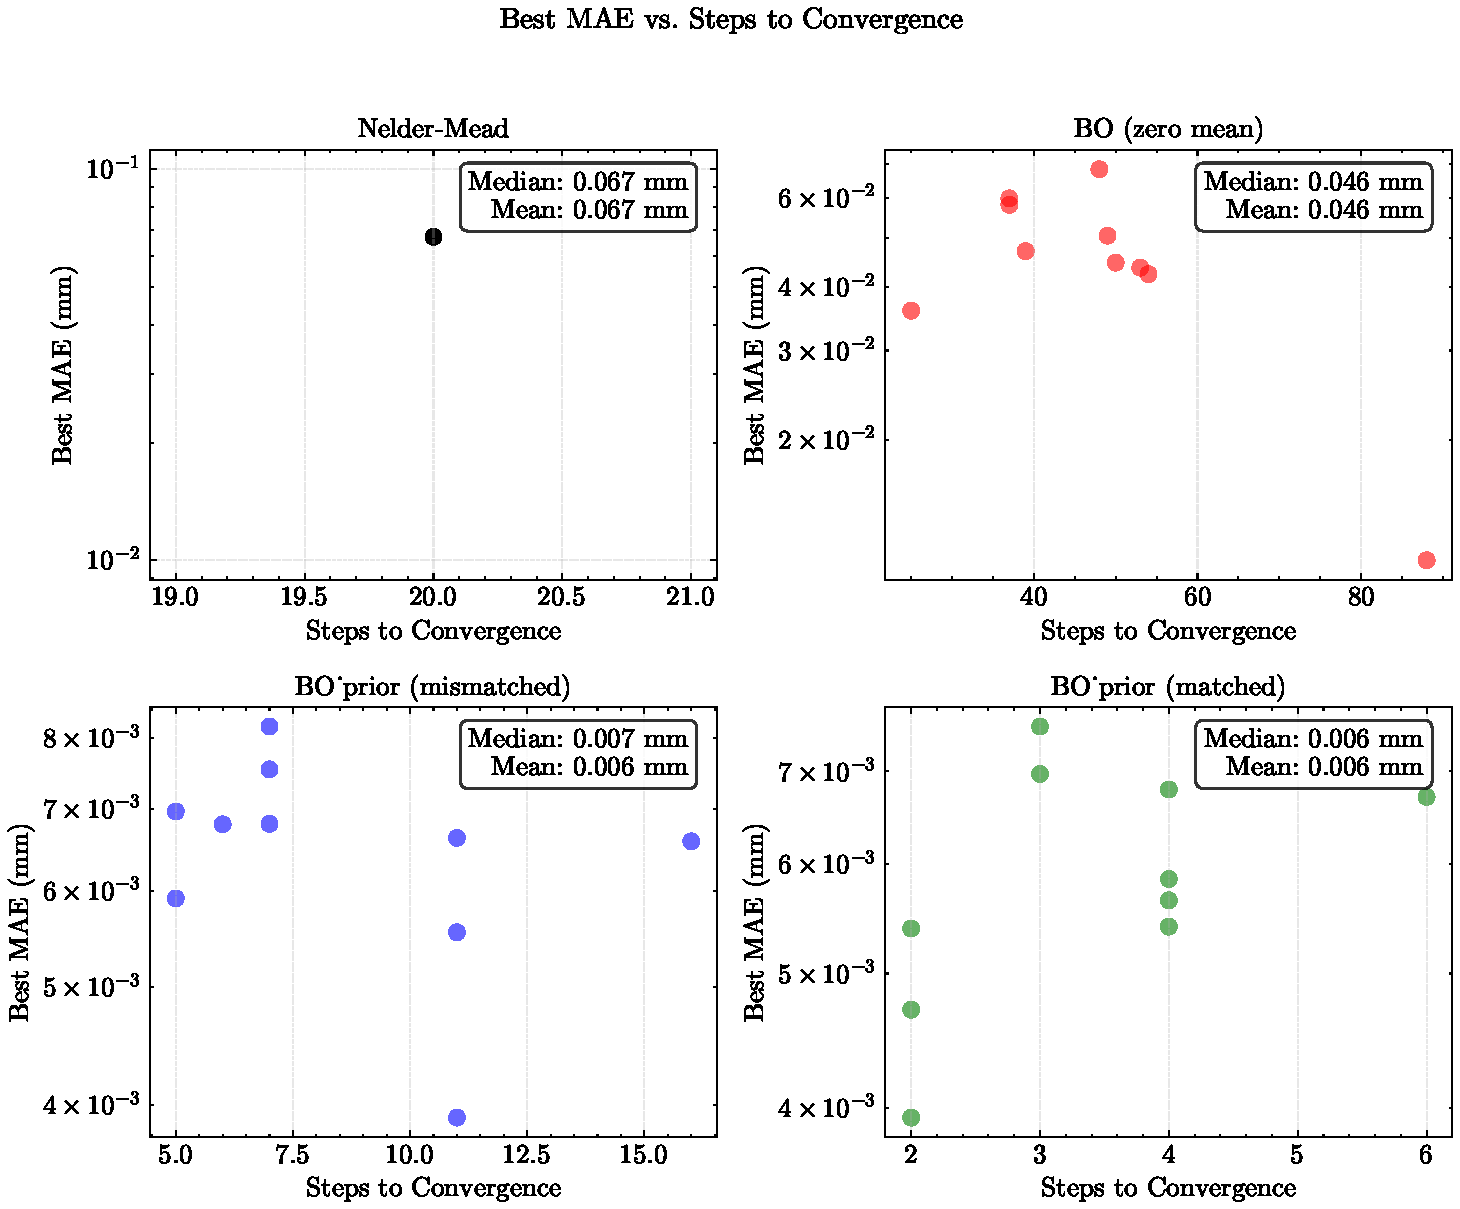
\includegraphics[width=0.8\textwidth]{figures/mae_vs_convergence.pdf}
    \caption{Final MAE versus steps to convergence for each trial, shown per method. Points in the bottom-left corner represent the ideal outcome: fast convergence to a lowerror. Note the logarithmic y-axis.}
    \label{fig:scatter_steps_vs_mae}
\end{figure}

The bottom left corner of each panel is where we want to be because this shows that this trial found a good solution quickly, 
while a dot on the top right means that this trial took a long time and still ended up with poor results. The Nelder-Mead panel 
has all its dots clustered top-right stalling near 67$\mu$m after about 94 steps (slow and poor), Standard BO is scattered 
across the middle with no clear link between convergence speed and final quality, this suggests that its unpredictable, 
some trials get lucky, some don’t, so it mostly depends on where the early random samples land whereas both physics informed 
prior based methods, consistently reach errors at or below 10$\mu$m. The matched prior scenario, most of them cluster on the 
left side, converging within 5-30 steps. Because the physics model is already accurate from the start. The y axis spans only 
4$\mu$m to 7$\mu$m, which means that every single trial lands on a great solution, the a few dots further to the right 
(around step 60 and 80) are the trials where the GP kept fiddling with tiny improvements (like going from 5.8 $\mu$m to 5.3 $\mu$m), 
but the final answer is just as good as fast trials. And finally for BO prior mismatched scenarios, the blue dots are spread more 
widely on the x axis (from step 15 to 90) but this makes sense because some trials figure out the misalignments quickly while 
some take longer. But even here the important thing is that at y axis, even the slowest trials still end up between 5$\mu$m to 10$\mu$m. 
The one dot near 10$\mu$m is likely a trial where the learned misalignments most probably did not quite meet the ground truth, 
but even that is still way better than anything what BO or Nelder-Mead achieved. 

\subsubsection{Misalignment Learning}
Whether the mismatched prior can recover the true quadrupole sets solely from the optimization data is a crucial concern. 
Lets recall that the ground truth misalignments range from zero to 0.3 mm with both positive and negative offsets, 
while the prior starts with all six values set to zero. By the end of the optimization process, the learnt misalignments 
values for each of the ten trials closely match the ground truth, despite starting from zero, confirming that the GP’s 
fitting is really able to pick up and collect more data. The estimates tend to settle around iteration 15, which is actually 
roughly the same point where the mismatched prior catches up with the matched prior scenario in the convergence curve.

\subsection{Discussion}
All the results and findings portray a consistent picture that Cheetah-based physics prior delivers a significant improvement 
across every metric, not just in how good the final solution is, but also in how quickly and reliably the optimiser gets there. 
There are several points worth discussing:
\begin{enumerate}
    \item The GP is given a warm start by the prior mean function, meaning that its predictions already approximate the shape of the true objective. This means that acquisition functions can make intelligent decisions from very first iterations, rather than going through several steps of  random exploration. The conversion curve plot makes this especially clear that physics informed methods are already below 100micrometre by 5 iteration, but standard BO takes upto iteration 60 or later.
    \item One might expect mismatched prior BO to perform significantly worse than matched one due to the completely incorrect misalignment values given to it. Whereas, the gap is quite small where the median final errors are identical (6$\mu$m), and the mismatched prior only requires approximately 10 extra steps to attain the 40$\mu$m target (14 vrs 4). This robustness is encouraged, as real world deployments often involve some degree of mismatch too.
    \item Though standard BO does eventually find solutions between 30$\mu$m and 60$\mu$m with two out of ten trails falling below 40$\mu$m, but a 20\% success rate and a median convergence of 82 steps to target are not practical for accelerators where the beam is expensive and operators need reliable tuning within few minutes. Whereas the physics based approaches tackle both concerns.
    \item The fact that Nelder-Mead converges to the same point in every trial (zero standard deviation on the final error) indicates a local minimum instead of a global one. In a 5 dimensional space with multiple local minima, this is not unexpected from a simplex based method. Thus, this local minimum (67$\mu$m) is not considered acceptable in practice as it exceeds the 40$\mu$m threshold.
    \item Compared to the original FODO demonstration \cite{kaiser2024bridging}, which was a two dimensional problem with a single learnable parameter, this project work used a 5 dimensional landscape with 6 learnable parameters. Still the methods with physics informed prior converged well in approximately 15 steps (mismatched) or 4 steps (matched). This shows that the approach scales reasonably well with the problem dimensionality in this scenario. 
\end{enumerate}

